\begin{figure}[htbp]
\centering
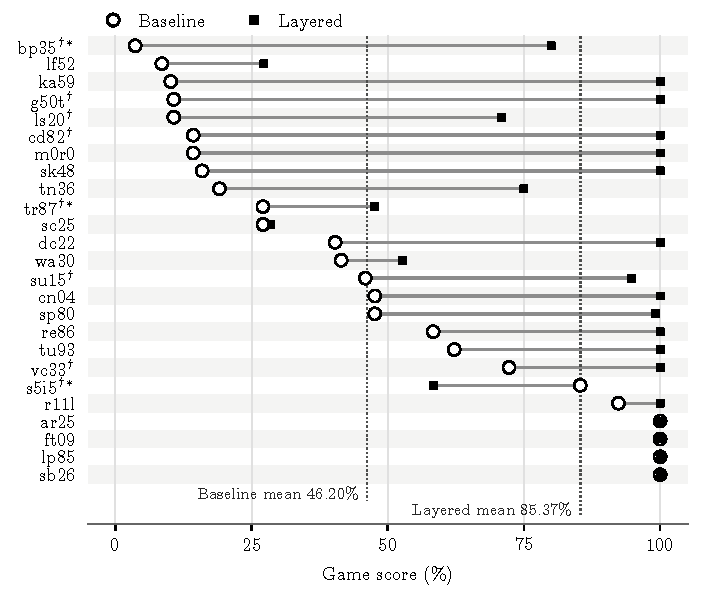
\includegraphics[width=0.66\linewidth]{figures/per_game_scores.pdf}
\caption{\textbf{The layered run scored higher than the baseline run in 20 of 25 games, the same in four, and lower in one.} Each row compares one baseline run and one layered run on the same game, under the same action cap. The rows run from the lowest baseline score to the highest. Open circles show the baseline score, filled squares show the layered score, and a line connects the two. The dotted lines mark the two mean scores. A dagger marks games used or studied during development. An asterisk marks layered runs stopped by repeated timeouts; the figure reports their scores at the point they stopped. The connecting lines show differences between two recorded runs; they do not show statistical uncertainty. Figure~\ref{fig:per-game-outcomes} adds levels completed and actions used.}\label{fig:per-game-scores}
\end{figure}
